\documentclass[10pt,a4paper, ngerman]{beamer}

\usepackage[ngerman]{babel}
\usepackage[T1]{fontenc}
\usepackage[utf8]{inputenc}
\usepackage{varioref}
\usepackage{hyperref}
\usepackage{cleveref}
\usepackage{amsmath}
\usepackage{amsfonts}
\usepackage{amssymb}
\usepackage{makeidx}
\usepackage{graphicx}
\usepackage{csquotes}
\usepackage{listings}
\usepackage{color}
\usepackage{xcolor}
\usepackage[most]{tcolorbox}
\usepackage{amssymb}
\usepackage{lmodern}
\usepackage{verbatim}

% Umlaute und ß in Listings
\lstset{basicstyle=\ttfamily}
\lstset{literate=%
  {Ö}{{\"O}}1
  {Ä}{{\"A}}1
  {Ü}{{\"U}}1
  {ß}{{\ss}}1
  {ü}{{\"u}}1
  {ä}{{\"a}}1
  {ö}{{\"o}}1
}

% Farben für Listings
\definecolor{codegreen}{rgb}{0,0.6,0}
\definecolor{codegray}{rgb}{0.5,0.5,0.5}
\definecolor{codepurple}{rgb}{0.58,0,0.82}
\definecolor{backcolour}{rgb}{0.95,0.95,0.92}
 
\lstdefinestyle{mystyle}{
    backgroundcolor=\color{backcolour},   
    commentstyle=\color{codegreen},
    keywordstyle=\color{magenta},
    numberstyle=\tiny\color{codegray},
    stringstyle=\color{codepurple},
    basicstyle=\footnotesize,
    breakatwhitespace=false,         
    breaklines=true,                 
    captionpos=t,                    
    keepspaces=true,                 
    numbers=left,                    
    numbersep=5pt,                  
    showspaces=false,                
    showstringspaces=false,
    showtabs=false,                  
    tabsize=2,
	language=[LaTeX]{TeX}
}

\lstset{style=mystyle}

\definecolor{hbbkBlueish}{HTML}{5e7b87}
\definecolor{hbbkReal}{HTML}{1A4354}
\setbeamercolor{logo}{bg=white}  %controls the color of the logo area
\setbeamercolor{author in sidebar}{fg=white} 
\setbeamercolor{palette primary}{bg=hbbkBlueish,fg=white}
\setbeamercolor{palette secondary}{bg=hbbkBlueish,fg=white}
\setbeamercolor{palette tertiary}{bg=hbbkBlueish,fg=white}
\setbeamercolor{palette quaternary}{bg=hbbkBlueish,fg=white}
\setbeamercolor{structure}{fg=hbbkBlueish} % itemize, enumerate, etc
\setbeamercolor{section in toc}{fg=hbbkReal} % TOC sections
\setbeamertemplate{navigation symbols}{}%remove navigation symbols



\usetheme{PaloAlto}
\renewcommand{\footnotesize}{\small}
\newcommand{\pftn}[1]{\let\thefootnote\relax\footnotetext{\tiny #1}}
\newcommand{\ftn}[2]{\footnote[#1]{\tiny #2}}
\newenvironment{hlbox}{\begin{tcolorbox}[enhanced,colback=white,colframe=white,sharpish corners,fuzzy halo=0.5mm with lightgray]}{\end{tcolorbox}}

\logo{
\includegraphics[width=0.155\linewidth]{hbbk-logo}}



\AtBeginSection{\frame{\frametitle{Gliederung}\tableofcontents[currentsection]}}

\setbeamercovered{transparent}
\author{Luca Kiebel \and Paul Hermann}
\title{Währungen und Internationale Zusammenarbeit}
%\subtitle{subtitle}
\date{\today}
\institute[HBBK]{Hans-Böckler-Berufskolleg}
\setlength{\itemsep}{10pt}
\begin{document}
\begin{frame}
\titlepage
\end{frame}

\section{Begriffsklärung}
\subsection{Was ist Währung?}
\begin{frame}{Was ist Währung?}{Begriffsklärung}
\pftn{http://bit.ly/2EShb0r{,} "Währung und internationale Zusammenarbeit"{,} Seite 226}
\begin{itemize}
\item Verfassung und Ordnung des Geldwesens eines Staates \pause
\item Allgeimer Sprachgebrauch: Geldeinheit eines Staates \pause
\item  Werden durch Abkürzungen oder Währungssymbole dargestellt 
\end{itemize}
\end{frame}

\subsection{Was sind Devisen?}
\begin{frame}{Was sind Devisen?}{Begriffsklärung}
\begin{itemize}
		\item Zahlungsmittel in fremder Währung\ftn{1}{https://www.duden.de/rechtschreibung/Devise} \pause
		\item Meist in Form von Guthaben bei ausländischen Banken\ftn{2}{https://de.wikipedia.org/wiki/Devisen}
\end{itemize}
\end{frame}

\subsection{Was ist der Wechselkurs?}
\begin{frame}{Was ist der Wechselkurs?}{Begriffsklärung}
\pftn{http://bit.ly/2EShb0r{,} "Währung und internationale Zusammenarbeit"{,} Seite 226}
\begin{itemize}
\item Das Austauschverhältnis zwischen zwei Währungen \pause
\item Richtet sich nach Angebot und Nachfrage
\end{itemize}
\end{frame}

\subsection{Was sind Primär- und Sekundäreinkommen?}
\begin{frame}{Was sind Primär- und Sekundäreinkommen?}
\begin{itemize}
\item Das Primäreinkommen ergiebt sich aus dem Marktprozess.\ftn{1}{http://wirtschaftslexikon.gabler.de/Definition/primaereinkommen.html} \pause
\item Sekundäreinkommen \ftn{2}{http://bit.ly/2EShb0r{,} "Währung und internationale Zusammenarbeit"{,} Seite 241}
\end{itemize}
\end{frame}

\section{Wechselkurse}
\subsection{Feste Wechselkurse}
\begin{frame}{Feste Wechselkurse}{Wechselkurse}
\begin{itemize}
\item Interventionen am Devisenmarkt halten Feste Wechselkurse aufrecht \pause
\item Angebot wird Nachfrage angepasst \pause
\item => Die Zentralbanken müssen eigene Geldpolitik auf Geldstabilität ausrichten
\end{itemize}
\pftn{http://bit.ly/2EShb0r{,} "Währung und internationale Zusammenarbeit"{,} Seite 230}
\end{frame}

\subsection{Flexible Wechselkurse}
\begin{frame}{Flexible Wechselkurse}
\pftn{http://bit.ly/2EShb0r{,} "Währung und internationale Zusammenarbeit"{,} Seite 231}
\begin{itemize}
\item Die meisten Währungen haben heute flexible Wechselkurse \pause
\item Angebot und Nachfrage \pause
\item Exporteure können mit Derivaten Wechselkursrisiken eingrenzen
\end{itemize}
\end{frame}

\section{Europäisches Währungssystem}
\subsection{von '79 bis '98}
\begin{frame}{Europäisches Währungssystem von  '79 bis '98}
\pftn{http://bit.ly/2EShb0r{,} "Währung und internationale Zusammenarbeit"{,} Seite 234}
\begin{itemize}
\item Vereinbarung für Leitkurse mit geringen Schwankungen \pause
\item Zentralbanken verpflichtet zu intervenieren
\end{itemize}
\end{frame}

\subsection{ab '98}
\begin{frame}{Europäisches Währungssystem ab '98}
\pftn{https://de.wikipedia.org/wiki/Wechselkursmechanismus\_II}
\begin{itemize}
\item Stabilisierung des gemeinsamen Binnenmarktes \pause
\item Schwankungsgrenzen von 15 \%
\end{itemize}
\end{frame}

\section{Zahlungsbilanz}
\begin{frame}{Zahlungsbilanz}
\begin{figure}
\centering
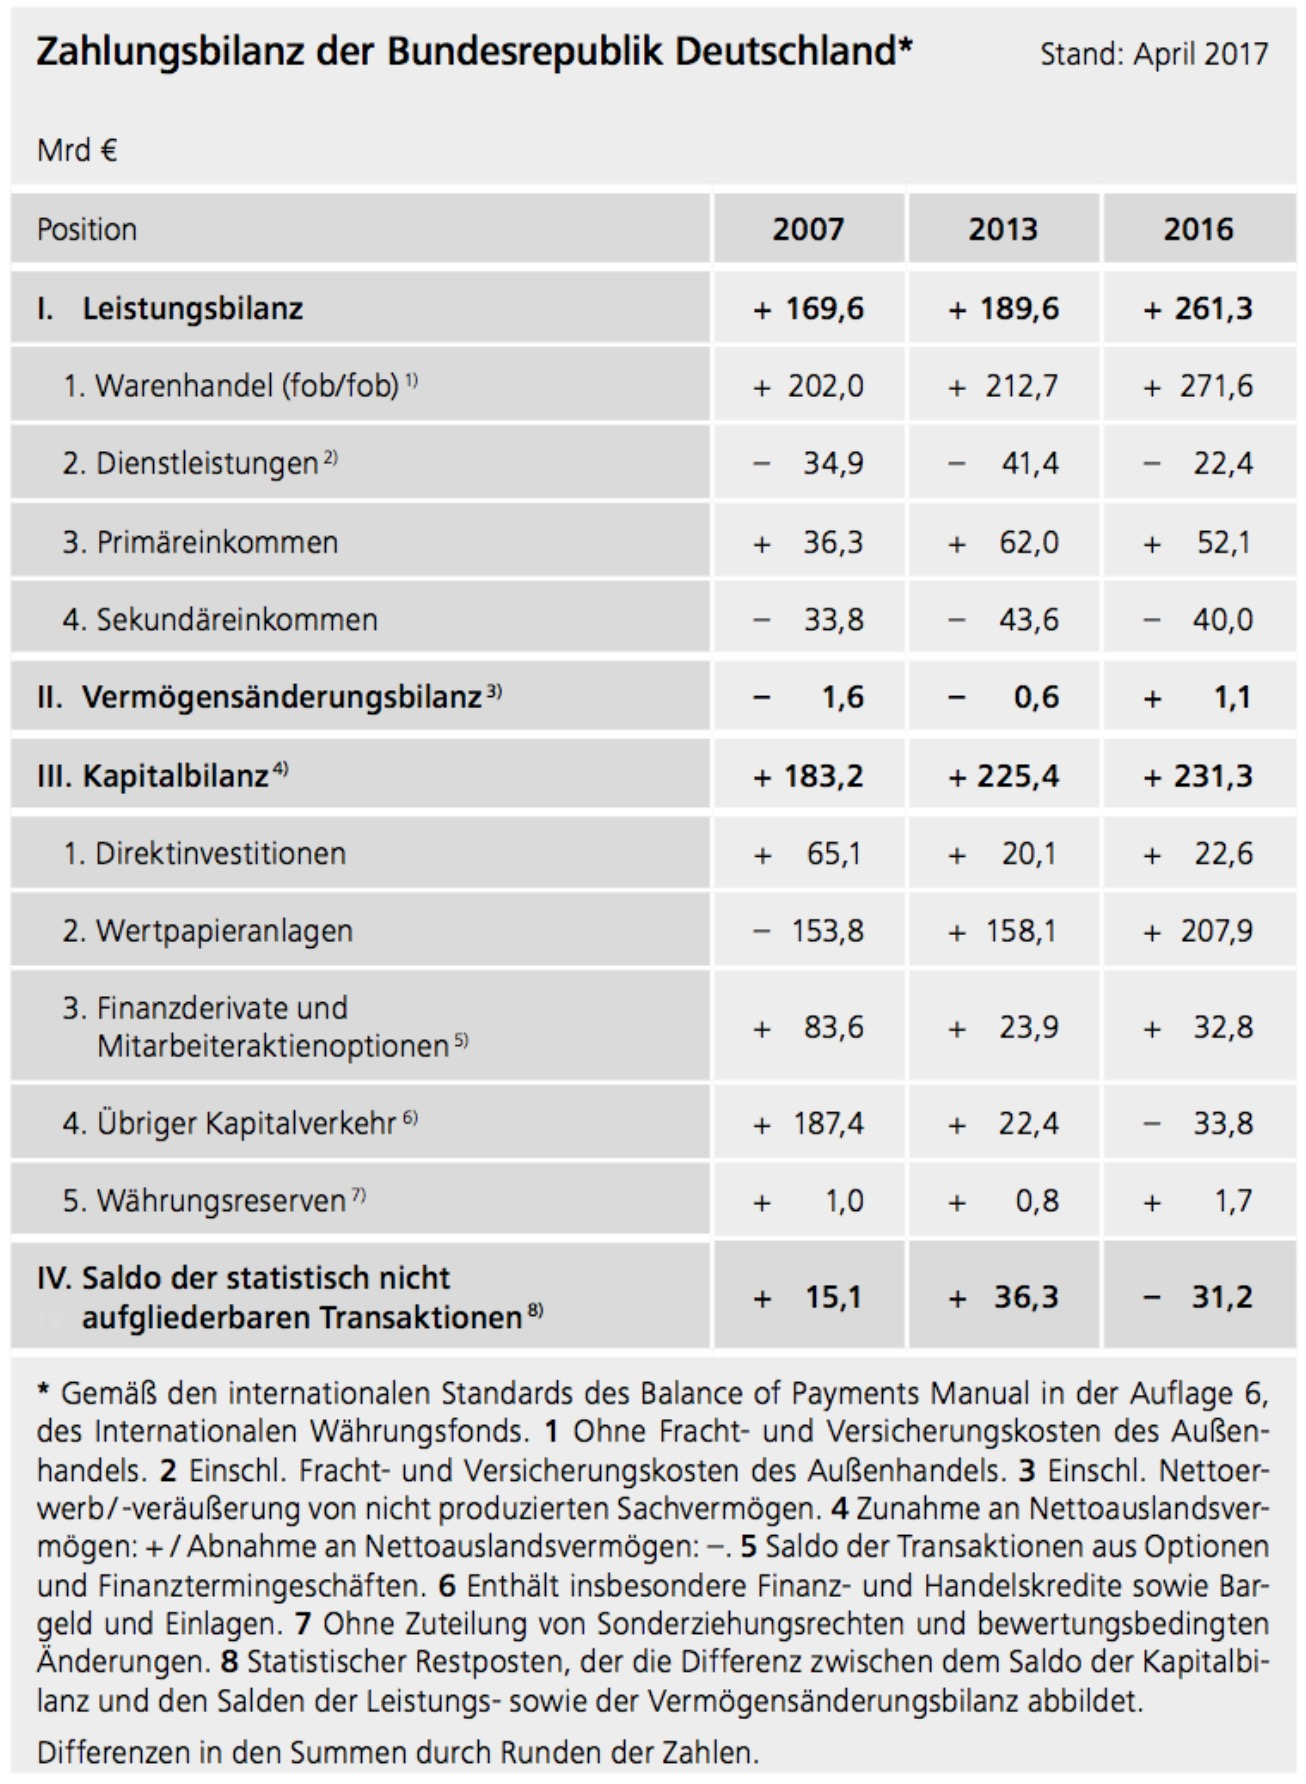
\includegraphics[height=0.9\textheight]{zahlungsbilanz_de}
\pftn{http://bit.ly/2EShb0r{,} "Währung und internationale Zusammenarbeit"{,} Seite 237}
\end{figure}
\end{frame}

\begin{frame}
\titlepage
\end{frame}

\end{document}